% Created by tikzDevice version 0.12.6 on 2025-04-07 11:41:10
% !TEX encoding = UTF-8 Unicode
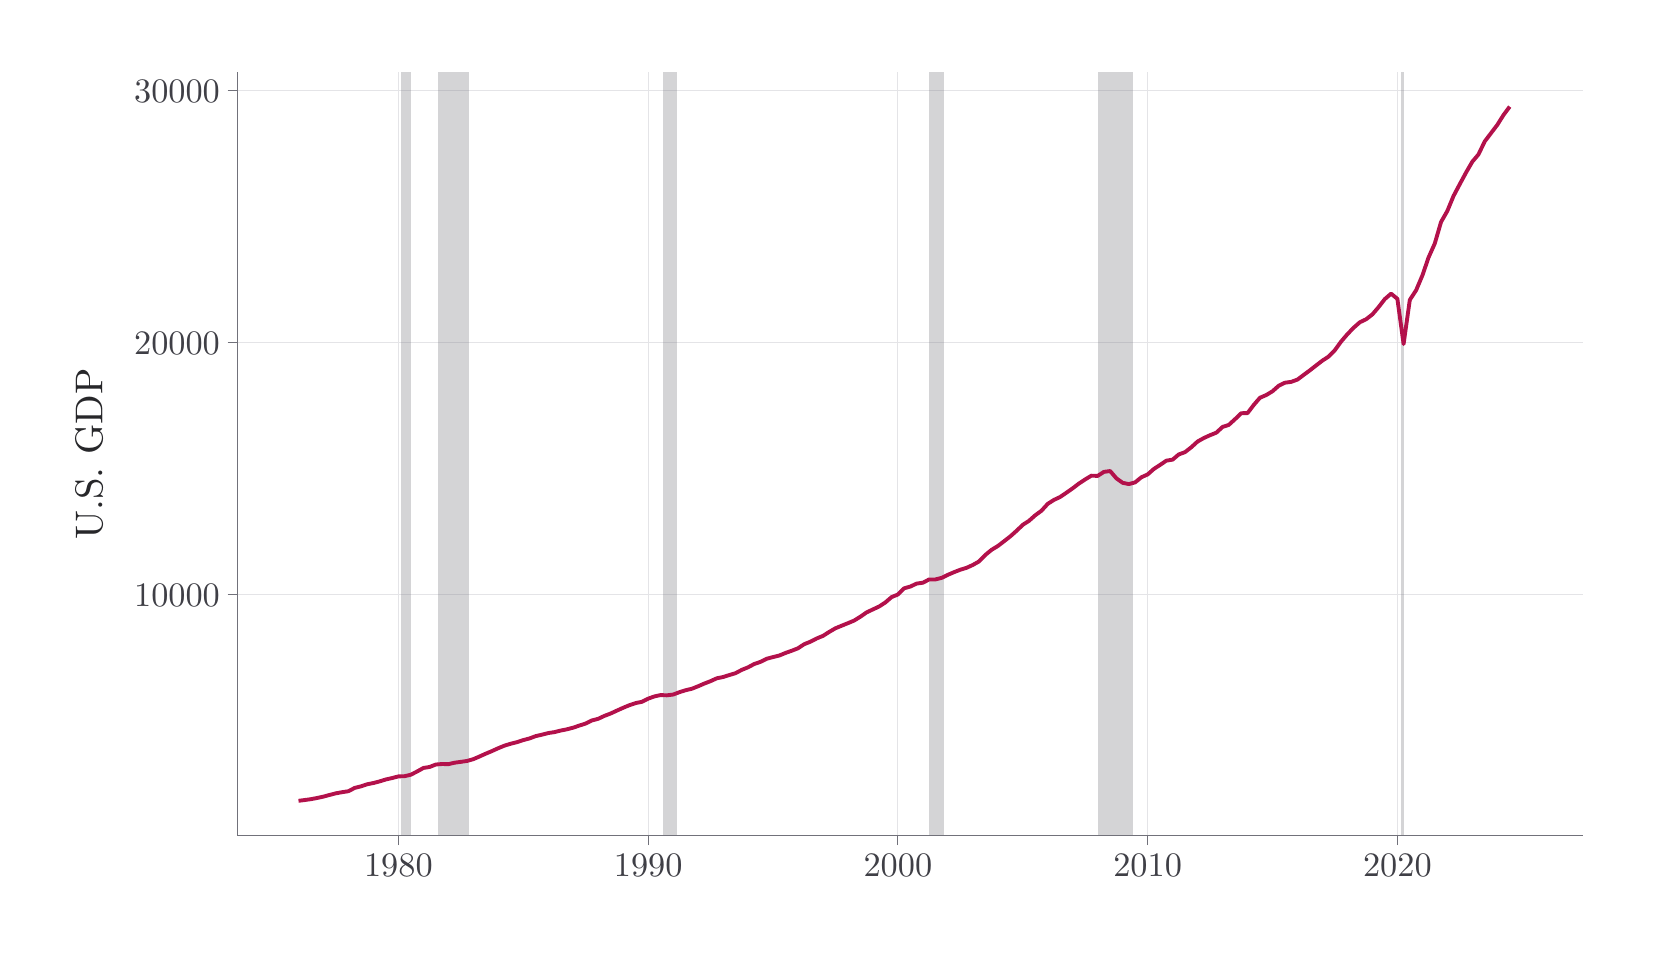
\begin{tikzpicture}[x=1pt,y=1pt]
\definecolor{fillColor}{RGB}{255,255,255}
\path[use as bounding box,fill=fillColor] (0,0) rectangle (578.16,325.21);
\begin{scope}
\path[clip] (  0.00,  0.00) rectangle (578.16,325.21);
\definecolor{drawColor}{RGB}{255,255,255}

\path[draw=drawColor,line width= 0.7pt,line join=round,line cap=round,fill=fillColor] (  0.00,  0.00) rectangle (578.16,325.21);
\end{scope}
\begin{scope}
\path[clip] ( 75.76, 33.29) rectangle (562.16,309.21);
\definecolor{drawColor}{RGB}{255,255,255}
\definecolor{fillColor}{RGB}{255,255,255}

\path[draw=drawColor,line width= 0.7pt,line join=round,line cap=round,fill=fillColor] ( 75.76, 33.29) rectangle (562.16,309.22);
\definecolor{drawColor}{RGB}{228,228,231}

\path[draw=drawColor,line width= 0.4pt,line join=round] ( 75.76,120.36) --
	(562.16,120.36);

\path[draw=drawColor,line width= 0.4pt,line join=round] ( 75.76,211.48) --
	(562.16,211.48);

\path[draw=drawColor,line width= 0.4pt,line join=round] ( 75.76,302.60) --
	(562.16,302.60);

\path[draw=drawColor,line width= 0.4pt,line join=round] (133.96, 33.29) --
	(133.96,309.21);

\path[draw=drawColor,line width= 0.4pt,line join=round] (224.22, 33.29) --
	(224.22,309.21);

\path[draw=drawColor,line width= 0.4pt,line join=round] (314.45, 33.29) --
	(314.45,309.21);

\path[draw=drawColor,line width= 0.4pt,line join=round] (404.70, 33.29) --
	(404.70,309.21);

\path[draw=drawColor,line width= 0.4pt,line join=round] (494.94, 33.29) --
	(494.94,309.21);
\definecolor{fillColor}{RGB}{113,113,122}

\path[fill=fillColor,fill opacity=0.30] (134.73, 33.29) rectangle (138.46,309.21);

\path[fill=fillColor,fill opacity=0.30] (148.24, 33.29) rectangle (159.53,309.21);

\path[fill=fillColor,fill opacity=0.30] (229.46, 33.29) rectangle (234.69,309.21);

\path[fill=fillColor,fill opacity=0.30] (325.72, 33.29) rectangle (331.00,309.21);

\path[fill=fillColor,fill opacity=0.30] (386.64, 33.29) rectangle (399.42,309.21);

\path[fill=fillColor,fill opacity=0.30] (496.42, 33.29) rectangle (497.18,309.21);
\definecolor{drawColor}{RGB}{179,17,75}

\path[draw=drawColor,line width= 1.4pt,line join=round] ( 97.87, 45.83) --
	(100.11, 46.12) --
	(102.36, 46.43) --
	(104.64, 46.87) --
	(106.91, 47.36) --
	(109.13, 47.97) --
	(111.38, 48.54) --
	(113.65, 48.96) --
	(115.93, 49.31) --
	(118.15, 50.49) --
	(120.40, 51.06) --
	(122.67, 51.81) --
	(124.94, 52.26) --
	(127.17, 52.85) --
	(129.42, 53.55) --
	(131.69, 54.06) --
	(133.96, 54.66) --
	(136.21, 54.73) --
	(138.46, 55.27) --
	(140.73, 56.44) --
	(143.01, 57.71) --
	(145.23, 58.06) --
	(147.48, 58.95) --
	(149.75, 59.13) --
	(152.02, 59.08) --
	(154.25, 59.60) --
	(156.50, 59.91) --
	(158.77, 60.24) --
	(161.04, 60.89) --
	(163.27, 61.85) --
	(165.51, 62.86) --
	(167.79, 63.82) --
	(170.06, 64.85) --
	(172.31, 65.78) --
	(174.56, 66.46) --
	(176.83, 67.04) --
	(179.10, 67.78) --
	(181.33, 68.37) --
	(183.57, 69.21) --
	(185.85, 69.73) --
	(188.12, 70.32) --
	(190.34, 70.66) --
	(192.59, 71.22) --
	(194.87, 71.68) --
	(197.14, 72.27) --
	(199.36, 73.03) --
	(201.61, 73.75) --
	(203.88, 74.87) --
	(206.16, 75.47) --
	(208.41, 76.53) --
	(210.65, 77.38) --
	(212.93, 78.44) --
	(215.20, 79.46) --
	(217.42, 80.38) --
	(219.67, 81.14) --
	(221.95, 81.61) --
	(224.22, 82.75) --
	(226.44, 83.55) --
	(228.69, 84.05) --
	(230.96, 83.95) --
	(233.24, 84.23) --
	(235.46, 85.07) --
	(237.71, 85.79) --
	(239.98, 86.32) --
	(242.25, 87.22) --
	(244.50, 88.20) --
	(246.75, 89.07) --
	(249.02, 90.11) --
	(251.30, 90.56) --
	(253.52, 91.28) --
	(255.77, 91.95) --
	(258.04, 93.15) --
	(260.32, 94.08) --
	(262.54, 95.27) --
	(264.79, 96.04) --
	(267.06, 97.17) --
	(269.33, 97.78) --
	(271.56, 98.32) --
	(273.81, 99.25) --
	(276.08,100.06) --
	(278.35,100.94) --
	(280.60,102.43) --
	(282.85,103.33) --
	(285.12,104.50) --
	(287.39,105.44) --
	(289.62,106.86) --
	(291.87,108.17) --
	(294.14,109.11) --
	(296.41,110.03) --
	(298.64,110.97) --
	(300.88,112.35) --
	(303.16,113.93) --
	(305.43,115.00) --
	(307.65,116.04) --
	(309.90,117.50) --
	(312.18,119.45) --
	(314.45,120.38) --
	(316.70,122.62) --
	(318.95,123.26) --
	(321.22,124.33) --
	(323.49,124.64) --
	(325.72,125.82) --
	(327.96,125.81) --
	(330.24,126.38) --
	(332.51,127.50) --
	(334.73,128.45) --
	(336.98,129.33) --
	(339.26,130.03) --
	(341.53,131.06) --
	(343.75,132.32) --
	(346.00,134.63) --
	(348.27,136.51) --
	(350.55,137.89) --
	(352.79,139.61) --
	(355.04,141.36) --
	(357.32,143.39) --
	(359.59,145.57) --
	(361.81,146.99) --
	(364.06,148.99) --
	(366.33,150.65) --
	(368.61,153.15) --
	(370.83,154.56) --
	(373.08,155.62) --
	(375.35,157.17) --
	(377.63,158.77) --
	(379.85,160.47) --
	(382.10,161.95) --
	(384.37,163.32) --
	(386.64,163.24) --
	(388.89,164.69) --
	(391.14,165.00) --
	(393.41,162.35) --
	(395.69,160.73) --
	(397.91,160.28) --
	(400.16,160.90) --
	(402.43,162.74) --
	(404.70,163.77) --
	(406.93,165.74) --
	(409.18,167.21) --
	(411.45,168.74) --
	(413.72,169.12) --
	(415.95,171.00) --
	(418.19,171.82) --
	(420.47,173.59) --
	(422.74,175.66) --
	(424.99,176.92) --
	(427.24,177.94) --
	(429.51,178.86) --
	(431.78,180.94) --
	(434.01,181.67) --
	(436.26,183.72) --
	(438.53,185.89) --
	(440.80,185.94) --
	(443.03,188.87) --
	(445.27,191.47) --
	(447.55,192.45) --
	(449.82,193.83) --
	(452.04,195.80) --
	(454.29,196.91) --
	(456.56,197.22) --
	(458.84,198.05) --
	(461.09,199.74) --
	(463.33,201.39) --
	(465.61,203.18) --
	(467.88,204.92) --
	(470.10,206.36) --
	(472.35,208.68) --
	(474.63,211.82) --
	(476.90,214.47) --
	(479.12,216.77) --
	(481.37,218.76) --
	(483.64,219.84) --
	(485.92,221.61) --
	(488.14,224.22) --
	(490.39,227.12) --
	(492.66,229.09) --
	(494.94,227.22) --
	(497.18,210.89) --
	(499.43,226.83) --
	(501.71,230.33) --
	(503.98,235.69) --
	(506.20,242.17) --
	(508.45,247.21) --
	(510.72,255.01) --
	(513.00,259.00) --
	(515.22,264.38) --
	(517.47,268.63) --
	(519.74,272.84) --
	(522.01,276.76) --
	(524.24,279.40) --
	(526.49,284.08) --
	(528.76,287.08) --
	(531.03,290.06) --
	(533.28,293.64) --
	(535.53,296.67);
\end{scope}
\begin{scope}
\path[clip] (  0.00,  0.00) rectangle (578.16,325.21);
\definecolor{drawColor}{RGB}{113,113,122}

\path[draw=drawColor,line width= 0.3pt,line join=round] ( 75.76, 33.29) --
	( 75.76,309.21);
\end{scope}
\begin{scope}
\path[clip] (  0.00,  0.00) rectangle (578.16,325.21);
\definecolor{drawColor}{RGB}{63,63,70}

\node[text=drawColor,anchor=base east,inner sep=0pt, outer sep=0pt, scale=  1.24] at ( 69.46,116.08) {10000};

\node[text=drawColor,anchor=base east,inner sep=0pt, outer sep=0pt, scale=  1.24] at ( 69.46,207.19) {20000};

\node[text=drawColor,anchor=base east,inner sep=0pt, outer sep=0pt, scale=  1.24] at ( 69.46,298.31) {30000};
\end{scope}
\begin{scope}
\path[clip] (  0.00,  0.00) rectangle (578.16,325.21);
\definecolor{drawColor}{RGB}{113,113,122}

\path[draw=drawColor,line width= 0.3pt,line join=round] ( 72.26,120.36) --
	( 75.76,120.36);

\path[draw=drawColor,line width= 0.3pt,line join=round] ( 72.26,211.48) --
	( 75.76,211.48);

\path[draw=drawColor,line width= 0.3pt,line join=round] ( 72.26,302.60) --
	( 75.76,302.60);
\end{scope}
\begin{scope}
\path[clip] (  0.00,  0.00) rectangle (578.16,325.21);
\definecolor{drawColor}{RGB}{113,113,122}

\path[draw=drawColor,line width= 0.3pt,line join=round] ( 75.76, 33.29) --
	(562.16, 33.29);
\end{scope}
\begin{scope}
\path[clip] (  0.00,  0.00) rectangle (578.16,325.21);
\definecolor{drawColor}{RGB}{113,113,122}

\path[draw=drawColor,line width= 0.3pt,line join=round] (133.96, 29.79) --
	(133.96, 33.29);

\path[draw=drawColor,line width= 0.3pt,line join=round] (224.22, 29.79) --
	(224.22, 33.29);

\path[draw=drawColor,line width= 0.3pt,line join=round] (314.45, 29.79) --
	(314.45, 33.29);

\path[draw=drawColor,line width= 0.3pt,line join=round] (404.70, 29.79) --
	(404.70, 33.29);

\path[draw=drawColor,line width= 0.3pt,line join=round] (494.94, 29.79) --
	(494.94, 33.29);
\end{scope}
\begin{scope}
\path[clip] (  0.00,  0.00) rectangle (578.16,325.21);
\definecolor{drawColor}{RGB}{63,63,70}

\node[text=drawColor,anchor=base,inner sep=0pt, outer sep=0pt, scale=  1.24] at (133.96, 18.42) {1980};

\node[text=drawColor,anchor=base,inner sep=0pt, outer sep=0pt, scale=  1.24] at (224.22, 18.42) {1990};

\node[text=drawColor,anchor=base,inner sep=0pt, outer sep=0pt, scale=  1.24] at (314.45, 18.42) {2000};

\node[text=drawColor,anchor=base,inner sep=0pt, outer sep=0pt, scale=  1.24] at (404.70, 18.42) {2010};

\node[text=drawColor,anchor=base,inner sep=0pt, outer sep=0pt, scale=  1.24] at (494.94, 18.42) {2020};
\end{scope}
\begin{scope}
\path[clip] (  0.00,  0.00) rectangle (578.16,325.21);
\definecolor{drawColor}{RGB}{39,39,42}

\node[text=drawColor,rotate= 90.00,anchor=base,inner sep=0pt, outer sep=0pt, scale=  1.40] at ( 27.00,171.25) {U.S. GDP};
\end{scope}
\end{tikzpicture}
